Der Raspberry Pi besitzt mit den \ac{GPIO} Pins eine Möglichkeit Sensoren anzusteuern. Nach der Dokumentation der Raspberry Pi Foundation\cite{GPIOMode77:online} können die \ac{GPIO} Pins 3.3V liefern und digitale Signale annehmen. Das neue Raspberry Pi 3 Modell hat den gleichen Aufbau der \ac{GPIO} Pins und die gleiche Pinbelegung. Schematisch wird die \ac{GPIO} Schnittstelle wie folgt dargestellt.
\begin{figure}[h]
	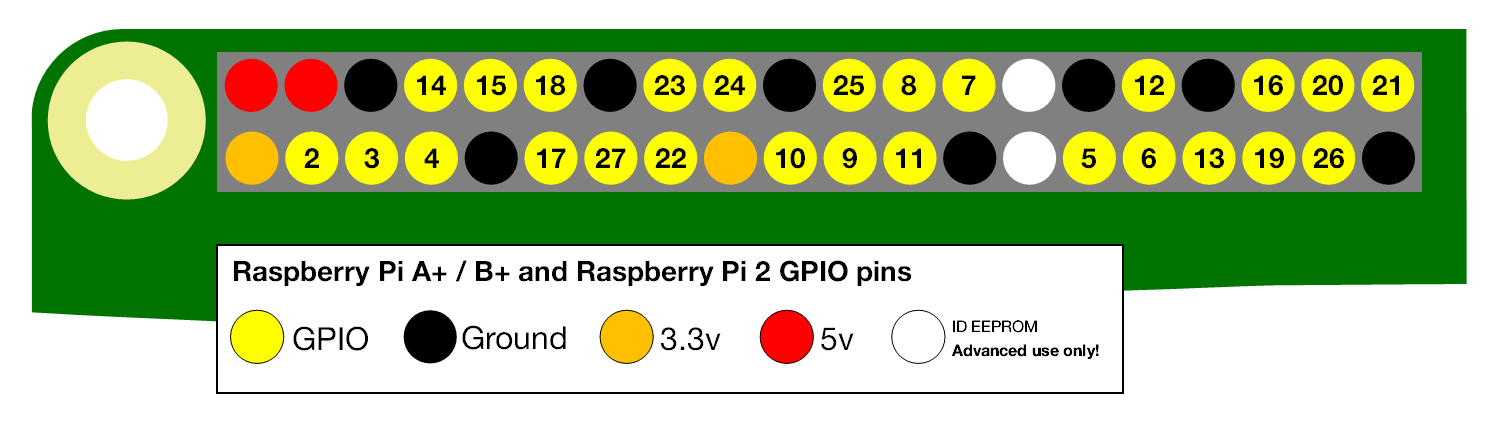
\includegraphics[width=\textwidth]{Bilder/Kapitel2/gpio_pins_pi2.png}
	\caption[Schema GPIO Pins]{Schematische Darstellung der GPIO Pins. Entnommen aus der Raspberry Pi Dokumentation\cite{GPIOMode77:online}.}
	\label{fig:Kapitel2/gpio_pins_pi2.png}
\end{figure}
\noindent
An den vorhandenen 3.3V und 5V Anschlüsse können Sensoren betrieben werden. Dennoch sind nicht alle Sensoren verwendbar. Der Raspberry Pi verfügt nur über die Möglichkeit digitale Signale an den \ac{GPIO} Pins zu verarbeiten. Es werden jedoch neben digitalen auch analoge Sensoren benötigt. Diese können nicht direkt an die Pins angeschlossen werden, aber das Problem wird mit einem \ac{A/D-Wandler} gelöst. \\
Die Erweiterungsplatine RPi-Explorer 700 von Joy-IT \cite{joyitrpi87:online} beinhaltet einen \ac{A/D-Wandler} an dem Analoge Pins angeschlossen werden können. Durch die Erweiterung ist es möglich bis zu vier analoge Sensoren an einem Sensorknoten betrieben werden. \\
Die \ac{GPIO} Schnittstelle unterstützt nur eine maximale Versorgungsspannung von 3.3V, was für die Sensoren ausreichend ist. Durch die Kompatibilität zum Arduino und dem Raspberry Pi können die Sensoren sowohl mit 5V als auch mit 3.3V betrieben werden.
Folgende Sensoren von Allnet\cite{111861pd90:online} werden  im \fullref{Verdrahtung_der_Sensoren} verwendet:
\begin{description}
\item[Temperatur und Luftfeuchtigkeitssensor] \hfill \\
	Der Sensor, KY-015, vom Typ DHT11 kann Temperaturen von 0 bis 50$^\circ$C mit einer Messungenauigkeit von $\pm$ 2$^\circ$C. Die Luftfeuchtigkeit kann im Bereich von 20 bis 95\% ($\pm$ 5\%) gemessen werden. Hierbei handelt es sich um einen digitalen Sensor.  
\item[Flammensensor]\hfill \\
	Der KY-026 besteht aus einer Fotodiode und einem \ac{Poti}. Die Fotodiode kann Wellenlängen im Bereich von etwa 720 - 1100 nm detektieren. Die Diode hat einen Erfassungswinkel von etwa 60$^\circ$. Der \ac{Poti} wird zur Empfindlichkeitseinstellung genutzt, somit kann eine Reichweite von etwa  ein bis sieben Metern abgedeckt werden. Der Sensor besitzt einen "'Digital Out"'-Pin, der high active geschalten wird. Sobald eine Flamme erkannt wird, liegt eine logische 1 auf dem Pin. Der "'Analog Out"'-Pin liefert ein analoges Signal, an welchem bei einer gemessenen Flamme eine niedrige Spannung anliegt.
\item[Lichtschranke]\hfill \\
	Das KY-010 Modul ist eine Lichtschranke, die beim Unterbrechen eine logische 1 an dem digitalen Ausgangspin liefert.
\item[Mikrofon]\hfill \\
	Das Mikrofon, KY-038, hat den gleichen Aufbau wie der Flammensonser. Im Gegensatz zum Flammensensor wird hierbei ein Mikrofonmodul, statt einer Fotodiode genutzt. Die Signale am Digital Out und Analog Out haben die gleiche Funktionalität wie beim Flammensensor. Dieses Modul dient hauptsächlich zur Detektion von kurzen aber lauten Tönen. Ein Anwendungsbeispiel hierfür ist eine Alarmfunktion. Beispielsweise kann das Zerbrechen eines Fensters festgestellt werden.
\item[Lichtsensor]\hfill \\
	Der Lichtsensor KY-018, bestehend aus einem Fotowiderstand, hat bei Dunkelheit einen Widerstand $>$20M$\Omega$ und bei Helligkeit $<$ 80$\Omega$. Damit kann bestimmt werden, ob in einem Zimmer das Licht brennt. Der Lichtsensor liefert ein analoges Signal.
\item[Schocksensor]\hfill \\
	Der Erschütterungssensor liefert eine logische 1 an dem Ausgangspin, falls eine Erschütterung festgestellt wurde. Das dient exemplarisch zur Umsetzung einer Schritterkennung am Boden.
\end{description}